\section{Background}

In this section, we introduce \BPGs{} through a real-world example, followed
by a discussion of related approaches.

%We first describe an example Best Practice Guidelines (\BPG{}) to
%explain characteristics that a \CIG{} language needs to have. We then
%explain limitations in existing approaches, and introduce our
%\emph{semantics-first} methodology.

%We first introduce relevant background work before discussing research challenges.
%In section \ref{subsec:cdss}, a real-world \BPG{} for management of sepsis
%in pediatric cases is used to introduce Guidelines-based \CDSSs{} and illustrate
%characteristics desirable of a framework for building \CDSSs{}.
%In section \ref{subsec:related-work}, we desribe progress
%made towards addressing said challenges by existing approaches and their limitations.
%Central to our approach is the \emph{semantics-first} philosophy,
%which is introduced in section \ref{subsec:semantics-first-and-k}.
%Section \ref{subsec:medik} introduces the \MediK{} \DSL{} for
%\emph{executable} \BPGs{} and explains how its design satisfies aforementioned
%characteristics. Section \ref{subsec:sepsis-cdss} discusses the \MediK{}-based
%\emph{executable} \BPG{} for management of sepsis and the corresponding \CDSS{}.

\subsection{Guidelines-based Clinical Decision Support Systems}\label{subsec:cdss}

We use a real-world \BPG{} for management of sepsis
in pediatric cases used at the Children's Hospital of Illinois at OSF St.
Francis Medical Center (OSF) to introduce \BPGs{} and Guidelines-based Clinical Decision
Support Systems (\CDSSs{}), and illustrate characteristics desirable of a framework for such system.
Sepsis is life-threatening condition caused by the body's extreme response to
an infection \cite{RhodesICM17}, and is
a major cause of morbidity and mortality in children \cite{Eisenberg2021JP}.
Adverse outcomes can, however, be mitigated through timely
identification and prompt treatment with antibiotics and
intravenous (IV) fluids \cite{Weiss2014CCM,Evans2018JAMA}.
\BPGs{} for screening and management of sepsis in pediatric Emergency
Departments (EDs) have shown effectiveness in screening and management of sepsis \cite{Eisenberg2021JP},
leading to their adoption in many pediatric EDs \cite{Balamuth2017EM,Sepanski2014FP}.

\begin{figure}
  \begin{subfigure}[b]{0.5\textwidth}
    \centering
    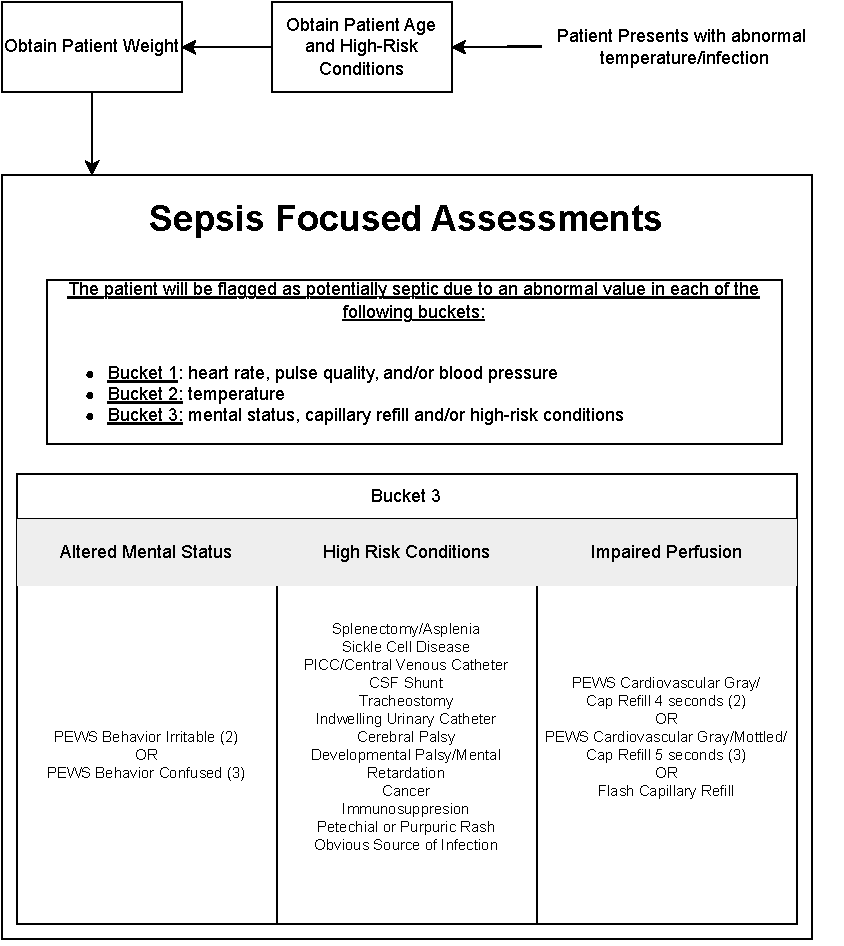
\includegraphics[width=0.65\textwidth]{sepsis-screening-osf}
    %\includegraphics[width=0.5\textwidth]{screening-vitals}
    \caption{Pediatric sepsis screening \BPG{}}\label{fig:sepsis-screening}
  \end{subfigure}
  \begin{subfigure}[b]{0.3\textwidth}
    \tiny
      \begin{tabular}{ | c || c | c | c | }
        \hline
        \textbf{Age}            & \textbf{Heart Rate}   & \textbf{Systolic BP} & \textbf{Temp}  \\
        \hline
        $0d - 1m$               & $>205$                & $<60$                & $<36 \text{ or } >38$ \\
        \hline
        $\geq 1m - 3m$          & $>205$                & $<70$                & $<36 \text{ or } >38$ \\
        \hline
        $\geq 3m - 1y$          & $>190$                & $<70$                & $<36 \text{ or } >38.5$ \\
        \hline
        $\dots$                 & $\dots$               & $\dots$              & $\dots$ \\
        \hline
        $\geq 13y$              & $>100$                & $<90$                & $<36 \text{ or } >38.5$ \\
        \hline
      \end{tabular}
      \caption{Vital Signs Chart}\label{table:vital-signs}
  \end{subfigure}
\end{figure}

In \figurename{} \ref{fig:sepsis-screening}, we present a simplified version of
the screening section of OSF's sepsis management guideline.
In essence, when a patient arrives at the
\ED{} with a fever or an infection, the \HCP{} is supposed to obtain
\begin{enumerate*}[label=(\alph*)]
  \item the patient's age,
  \item any conditions, such as cancer, immunosuppression, etc,
    that increase likelihood of sepsis, and
  \item the patient's vital signs, such as heart rate, systolic blood
    pressure, respiratory rate, etc.
\end{enumerate*}
This information is then used to check for abnormalities
in clusters of linked information, called \say{buckets}. For instance, if
the patient's heart rate is abnormal, then \say{bucket 1} is said to
have an abnormal value.
Checking for such abnormalities often involves the use of tables, such as
\tablename{} \ref{table:vital-signs}, that contain normal ranges indexed by
\emph{age}.
%\footnote{For brevity, we omit some age ranges and vital signs from table
%\ref{table:vital-signs}}.
If the patient has at least one abnormal value in every \say{bucket},
then he/she is flagged as potentially septic.

The \BPG{}-recommended treatment for
sepsis involves multiple concurrent workflows, such as
screening for septic shock, fluid resuscitation, and administering antibiotics.
In \figurename{} \ref{fig:fluid-therapy}, we provide
a version of the fluid resuscitation guideline used
at OSF. Briefly, if the patient is flagged as potentially septic, the guideline suggests
\begin{enumerate*}[label=(\roman*)]
  \item obtaining any fluid-overload risks,
  \item administering normal saline (typically over a period of 15 minutes),
    where the dosage is dictated by risks determined in previous step,
  \item assessing signs of fluid-overload,
  \item evaluating patient responsiveness to normal saline upon completion of
    the administering process, and,
  \item determining whether another fluid bolus should be administered based on
    information from previous steps.
\end{enumerate*}
\begin{figure}[b]
  \centering
  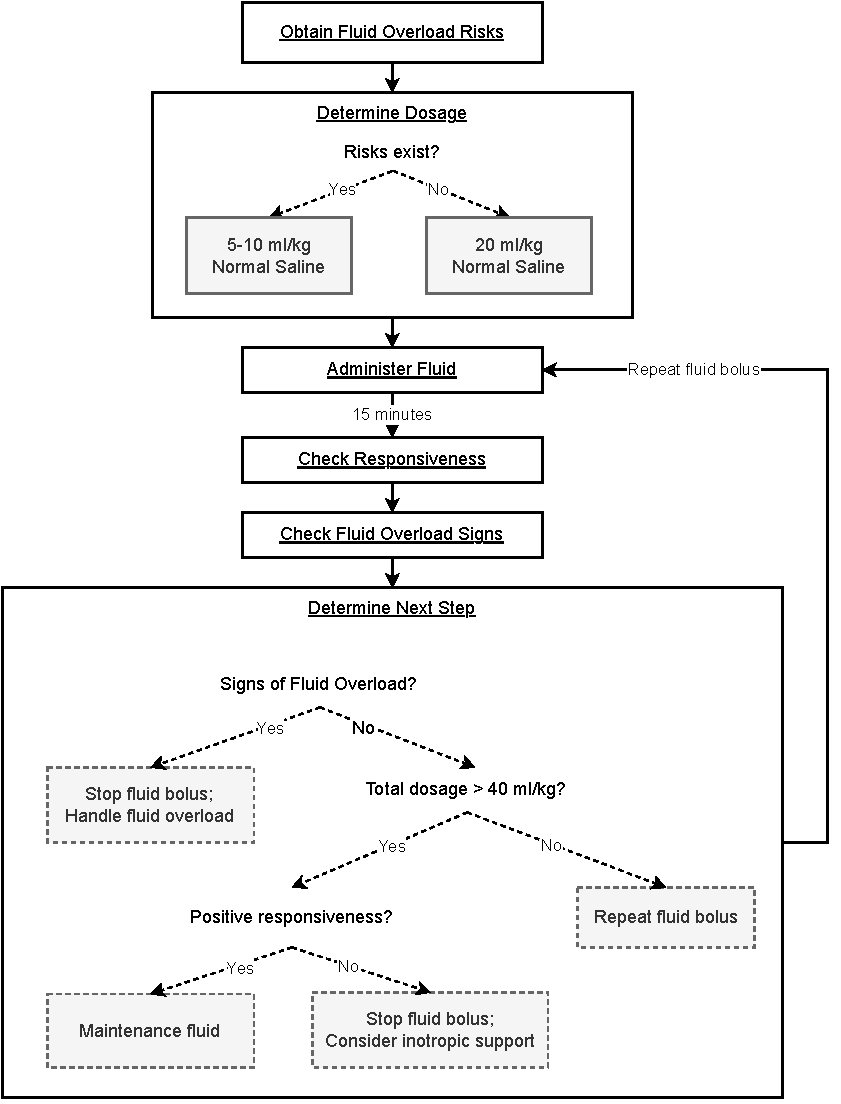
\includegraphics[scale=0.45]{FluidWorkflow-fmcad.pdf}
  \caption{Fluid Resuscitation Guideline}\label{fig:fluid-therapy}
\end{figure}

This real-world \BPG{} exhibits characteristics common
across many \BPGs{}. Specifically \BPGs{} typically:
\begin{itemize}
  \item Involve \stress{concurrent} workflows, such as administering drugs,
    monitoring vitals, performing treatment, etc. There may also be
    inter-workflow interactions. For instance, a diagnosis of sepsis during the
    screening may require modifications to an ongoing course antibiotics.
  \item Often specified in a \stress{flowchart-like}
    notation. See \cite{AHAFlowcharts} and \cite{CancerCareFlowcharts} for other flowchart-based \BPGs{} for management of \emph{cardiac arrest}, and
    screening, risk-reduction, treatment and survivorship in
    cancer care respectively.
  \item Require communication between \stress{heterogeneous agents} such as
     monitors and Electronic Health Records (EHRs).
  \item Often use \stress{tables} indexed by parameters such as age, weight,
    etc to present normal/abnormal ranges for measurements, or recommended dosages for drugs.
\end{itemize}

%\begin{center}
%\renewcommand{\arraystretch}{0.5}
%\setlength\extrarowheight{-9pt}
  \begin{table}
    \tiny
  \begin{tabularx}{\textwidth}{
      >{\centering\arraybackslash}X
    || >{\centering\arraybackslash}X
    | >{\centering\arraybackslash}X
    | >{\centering\arraybackslash}X
    | >{\centering\arraybackslash}X
    | >{\centering\arraybackslash}X
  }
                 & Specification-Implementation Gap  & Complex Workflows  & Diverse Agents   & Formal Analysis  & Holistic Safety  \\
    Arden Syntax & $\greencheck$                     & $\redcross$        & $\redcross$    & $\redcross$        & $\redcross$ \\
    GLIF         & $\greencheck$                     & $\greencheck$      & $\redcross$    & $\redcross$        & $\redcross$ \\
    Asbru        & $\greencheck$                     & $\greencheck$      & $\redcross$    & $\greencheck$      & $\redcross$ \\
    PROForma     & $\greencheck$                     & $\greencheck$      & $\redcross$    & $\redcross$        & $\redcross$ \\
    GLARE        & $\greencheck$                     & $\greencheck$      & $\redcross$    & $\cancelcheck$     & $\cancelcheck$ \\
    SAGE         & $\greencheck$                     & $\greencheck$      & $\greencheck$  & $\redcross$        & $\redcross$ \\
    Promela/SPIN & $\redcross$                       & $\greencheck$      & $\redcross$    & $\greencheck$      & $\cancelcheck$ \\
    AMSs         & $\redcross$                       & $\greencheck$      & $\redcross$    & $\greencheck$      & $\redcross$ \\
    P            & $\redcross$                       & $\greencheck$      & $\greencheck$  & $\greencheck$      & $\redcross$ \\
  \end{tabularx}
  \caption{Comparison of Existing Approaches}\label{table:existing-approaches}
  \end{table}
%\end{center}

\subsection{Related Work}\label{subsec:related-work}

Recall from section \ref{sec:introduction} the following
challenges in building \CDSSs{}:
\begin{itemize}
  \item \textbf{Specification-Implementation Gap:} The specification,
    i.e., the \BPG{}, may differ from its translation in a computable
    medium, i.e. \CIG{}.
  \item \textbf{Complexity:} \BPGs{} encode complex medical knowledge,
    involving multiple \emph{concurrent} workflows and \emph{inter-workflow}
    interactions. Moreover, $\CDSSs{}$ interact with \emph{diverse
    external agents} such as medical sensors and patient records.
  \item \textbf{Formal Analysis:} As \CDSSs{} are \emph{safety-critical},
    it's desirable to have execution engines with \emph{correctness guarantees}
    and a suite of formal analysis tools such as model checkers and deductive
    verifiers that can handle aforementioned complexity.
  \item \textbf{Holistic Safety:} A mechanism for establishing the safety
    of the entire system must exist. This includes reasoning about external
    components, and safely integrating AI-enabled components.
\end{itemize}

Existing research has been instrumental in both recognizing aforementioned
challenges and addressing them to various degrees, leading to greater \CDSS{}
adoption. In \tablename{} \ref{table:existing-approaches}, we provide an overview of
how existing work addresses aforementioned challenges. We use
\greencheck{}, \cancelcheck{}, and \redcross{} to depict that an approach
fully-addresses, partly-addresses, or doesn't address a limitation respectively.
We next go over notable approaches, and describe how they incrementally
address said challenges.

\paragraph{Arden Syntax:}

The Arden Syntax \cite{HripcsakCBM94} is a widely used medium for
writing executable \BPGs{}. First proposed in 1989, it was among the
first languages to recognize and address the \emph{specification-implementation
gap} by emphasizing \emph{comprehensibility} to non-experts in Computer Science \cite{SamwaldJBI12}.
Guidelines are described using Medical
Logic Modules that contains information related to guideline's purpose
, maintenance, and medical knowledge. The modules are modular to allow
re-use and sharing across hospitals. But, Arden Syntax
is focused on describing simple, modular, and independent
guidelines (such as reminders), and not on guidelines with complex logic (such
as treatment protocols) \cite{PelegJBI01}.

\paragraph{GLIF:}

Arden Syntax's limitation in modeling complexity is addressed by
GLIF \cite{BoxwalaJBI04}: a language that uses flowcharts to expressed
guidelines. A multi-level approach is
employed to manage complexity: at the top is the conceptual level, where
only high-level details relevant for human-comprehension are present. In the
middle is a computable-level, where details of guideline execution flow
and patient data elements are specified. At the bottom is the implementable
level, where institution-specific details and mappings into patient data are
specified. Both Arden Syntax and GLIF  eliminate
the gap between the \BPG{}, i.e. the specification, and the \CIG{}, i.e. implementation as
they're meant to be either directly used by clinicians (or in collaboration with
computer scientists) to express \BPGs{} in an executable medium. \CIGs{}
expressed in them are meant to be shared across hospitals, and are thus modular.
However, neither formalism has complete formal semantics, or comprehensive support for
rigorous formal analysis.

\paragraph{Asbru:}

The need for formal analysis is identified by Asbru: a formalism with formally
defined syntax and semantics \cite{ShaharAMIA96}. In Asbru, a guideline is modeled as a plan
that contains:
\begin{enumerate*}[label=(\roman*)]
  \item intentions that define aims,
  \item conditions that specify when the plan is applicable,
  \item effects that define expected behavior during execution, and,
  \item a body containing other sub-plans.
\end{enumerate*}
Apart from an execution engine, the Asbru ecosystem also contains
other tools, such as a model checker for verification \cite{BaumlerSPIN06}.
However, the formal semantics of Asbru have been only partially defined, and
is insufficient to implement tools for the language \cite{SuttonAMIA03}.

\paragraph{PROForma:}

The importance of a complete formal-semantics is identified and addressed
by PROforma \cite{SuttonAMIA03}, another formalism that uses plans to
model guidelines. A PROforma plan is made of a sequence of tasks.
The plan defines constraints on their enactment, and circumstances
for termination (for example, exceptions) \cite{SuttonAMIA03}. But, despite
having complete formal semantics, it does not have a comprehensive suite of
formal analysis tools such as model checkers, deductive verifiers.

\paragraph{SAGE:}
The SAGE guideline model \cite{TuSAGE04} uses the Prot\'eg\'e knowledge
representation framework \cite{NoyAMIA03} to model guidelines,
and improves on aforementioned approaches by
enabling seamless integration into hospitals' existing Clinical Information Systems
(\CISs). But, it lacks complete formal semantics, and analysis tools
such as deductive verifiers and model checkers.
The GLARE formalism \cite{TerenzianiBook04} uses an actions based approach
to represent guidelines, and addresses clinician-comprehensibility and
modularity. For formal analysis, GLARE guidelines can be translated to
Promela: the SPIN model checker's specification language \cite{GiordanoAMIA06}.
The approach partly addresses holistic safety as
external agents (such as clinicians) can be modelled and analyzed.
But, the scenario where the external agent's behavior
deviates from the model during system execution isn't addressed.


Languages outside the medical domain can also be used to reason about
medical systems. For example, in \cite{ArcainiMEMCODE15}, Abstract State
Machines (\ASMs) are used to validate and verify a system for measuring
patients' stereoacuity in the diagnosis of amyblyopia.
Along similar lines, the P language \cite{DesaiPLDI13}
and analysis of large concurrent systems provides a convenient medium
for expressing multiple workflows and interactions as concurrently
executing Finite State Machines (FSMs). External agents can be modeled
using \emph{ghost} that are used for formal analysis, but discarded at runtime.
But such formalisms, while suitable for formal verification, may
not be easily comprehensible to clinicians for validation.

This proposal aims to build on progress made by existing work to
address aforementioned challenges using the \emph{semantics-first} approach,
which we describe in the following section.

\subsection{Semantics-First Approach and the $\K$ Framework}\label{subsec:semantics-first-and-k}
\begin{wrapfigure}{l}{0.6\textwidth}
  \centering
  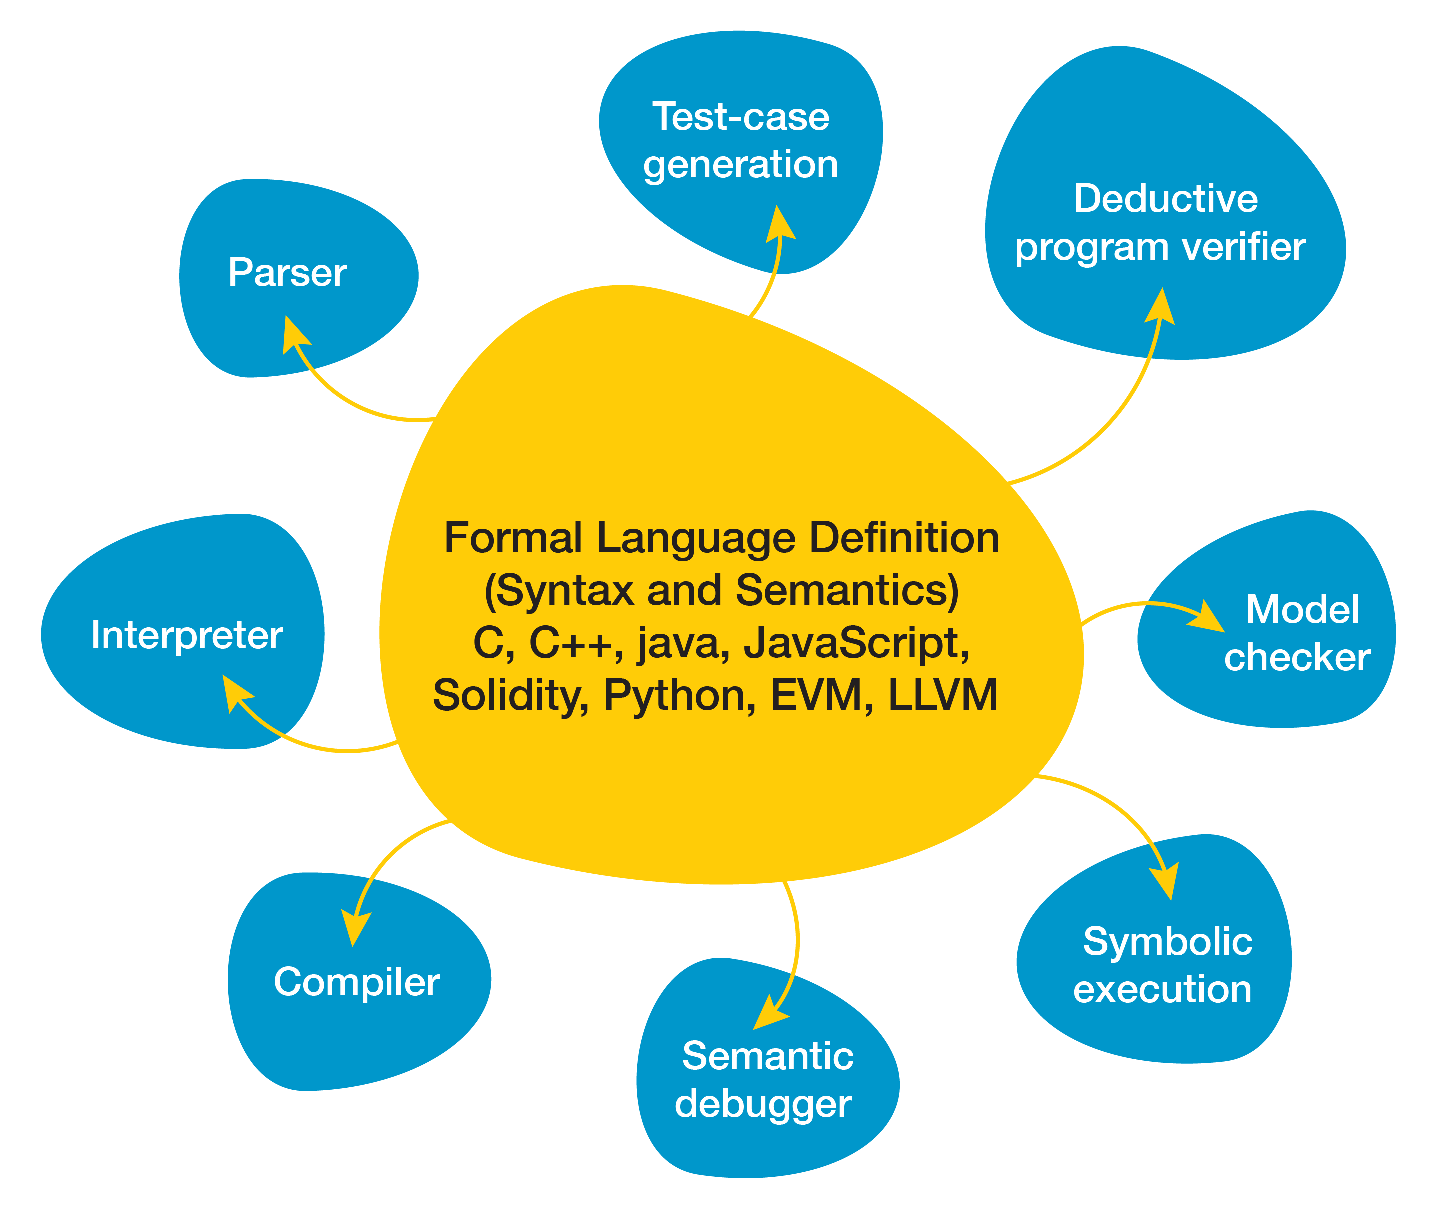
\includegraphics[width=0.5\textwidth]{k-overview}
  \caption{\emph{Semantics-first} Approach} \label{fig:k-overview}
\end{wrapfigure}
Recall from section \ref{sec:introduction} that at the core of our approach
is a new \DSL{} for writing executable \BPGs{} called \MediK{}.
The \emph{semantics-first} approach dictates that instead of
implementing tools such as interpreters, model checkers and deductive verifiers
from scratch in an ad-hoc way, the semantics of the language should
be formally defined and utilized to derive said tools in a
\emph{correct-by-construction} fashion, as shown in \figurename{} \ref{fig:k-overview}.

For a language like \MediK{}, the semantics first approach has many benefits. First,
since \MediK{} is meant to be used in safety-critical settings,
it's vital that its interpreter has correctness guarantees and formal analysis
tools such as model checkers and deductive verifiers, which the approach ensures.
Second, \MediK{} has to evolve quickly to incorporate feedback that it receives from domain experts.
Had we implemented all tools from scratch, any update to the language would
require updates to the tools as well. With our approach, only the formal semantics
need updating. Since the tools are derived from the semantics, they reflect all
changes automatically.

\MediK{}'s semantics have been formalized in the $\K{}$-framework, which
we describe next. $\K$ is a rewrite-based executable semantics framework in which
programming languages can be defined
using configurations and rules \cite{KFrameworkURL}. Semantics
defined in $\K$ typically consist of the following three components:
\begin{itemize}
  \item \emph{Syntax:} Defined using BNF-like notation, and utilized
    by $\K{}$ to generate a parser for the language.
  \item \emph{Configuration:} Organizes the program execution state into
    units called \emph{cells} that be nested.
  \item \emph{Rules:} Operate over configuration segments and define
    program evolution via rewrites.
\end{itemize}

\begin{figure}[H]
  \centering
  \begin{lstlisting}[style=ksty, language=k,  multicols=2,
  basicstyle=\ttfamily\notsotiny, numbers=left
  ,showspaces=false
  ,xleftmargin=2em]
module IMP-SYNTAX
  imports DOMAINS-SYNTAX
  syntax Exp ::=
      Int
    | Id
    | Exp "+" Exp    [left, strict]
    | Exp "-" Exp    [left, strict]
    | "(" Exp ")"    [bracket]

  syntax Stmt ::=
      Id "=" Exp ";" [strict(2)]
    | "if" "(" Exp ")"
        Stmt Stmt    [strict(1)]
    | "while" "(" Exp ")" Stmt
    | "{" Stmt "}"   [bracket]
    | "{" "}"
    > Stmt Stmt      [left, strict(1)]
  syntax Pgm ::= "int" Ids ";" Stmt
  syntax Ids ::= List{Id,","}
endmodule
module IMP imports IMP-SYNTAX
  imports DOMAINS
  syntax KResult ::= Int
  configuration
   <T> <k> $PGM:Pgm </k>
       <state> .Map </state> </T>
  rule <k> X:Id => I ...</k>
       <state>... X |-> I ...</state>
  rule I1 + I2 => I1 +Int I2
  rule I1 - I2 => I1 -Int I2
  rule <k> X = I:Int ; => . ...</k>
       <state>... X |-> (_ => I) ...</state>
  rule {} S:Stmt => S
  rule if(I) S _ => S requires I =/=Int 0
  rule if(0) _ S => S
  rule while(B) S => if(B) {S while(B) S} {}
  rule <k> int (X, Xs => Xs) ; S </k>
       <state>... (. => X |-> 0) </state>
  rule int .Ids ; S => S
endmodule
\end{lstlisting}
  \caption{IMP Semantics in $\K$}\label{fig:imp-semantics}
\end{figure}

In \figurename{} \ref{fig:imp-semantics}, we provide the $\K$ semantics
for Imp, a simple imperative language that supports arithmetic expressions and
statements such as variable declaration and assignment, branching (\inlineimp{if}) and looping (\inlineimp{while}).
In $\K{}$ code must be placed inside a \inlinek{module}. The Imp definition
consists of two such modules: \inlinek{IMP-SYNTAX} (lines 1-20) defining the language's
syntax, and \inlinek{IMP-SEMANTICS} containing the \inlinek{configuration} (lines 24-26)
and rewrite rules (lines 27-39). Note that \inlinek{module IMP} imports
\inlinek{module IMP-SYNTAX}, allowing rules to utilize the language's syntax.

\emph{Syntax} in $\K{}$ is defined using BNF-like notation; terminals are enclosed
in quotes, and non-terminals begin with an uppercase. For example,
consider the declaration of Imp expressions on lines 3-8. On lines 4-5,
$\K$'s builtin support for integers (\inlinek{Int}) and program identifiers
(\inlinek{Id}) is used to support arithmetic expressions over program variables.
On lines 6 and 7, the attribute \inlinek{left} is used to declare the
corresponding operator as left associative. The \inlinek{strict} attribute is used
to assign \emph{evaluation strategies}. On lines 6 and 7, the attribute
signifies that both operand sub-expressions must be completely evaluted before the
before the operator (\inlinek{+}, \inlinek{-}) can be evaluted. Similarly, for
an assignment statement on line 12,
the \inlinek{strict(2)} indicates that the second argument, i.e., the
expression to the right of the \inlineimp{=} sign must be evaluated before
the identifier on the left of the \inlineimp{=} is updated. On line 17,
the \inlinek{>} signifies that block of \inlinek{Stmt} productions preceding
the sign (lines 11-16) have a higher precedence, i.e. bind tighter,
than the production on line 17.
On line 18, an Imp program is defined to start with a list of program variable
declarations (\inlinek{"int" Ids ";"}) followed by other statements, where
 \inlinek{List\{Id, ","\}} is used on line 19 to define \inlinek{Ids}, the comma-separated list of
program identifiers.

Once the \emph{syntax} has been defined, $\K$ can utilize it to generate a
parser for programs in the language. To impart semantics,
we must describe how the program's \emph{execution state} evolves during
execution. In $\K$ \emph{state} is organized into a \emph{configuration}.
The configuration is an unordered list of (potentially nested) \emph{cells},
specified using an XML-like notation. When writing \emph{rules} (as rewrites)
over this state, any subset of the \emph{cells} present in the configuration
can be mentioned. Thus, only parts of the state \emph{relevant} to the rule
need to be mentioned; the rest of the state is assumed to remain unchanged.
The keyword \inlinek{configuration} (line 24)  defines a \emph{configuration},
followed by xml-like notation for the $\K$ \emph{cells}. For instance,
\inlinek{<foo> <bar> ...  </bar> </foo>} corresponds to $\K$ \emph{cells} with
the names \inlinek{foo} and \inlinek{bar} respectively, where \inlinek{bar}
is nested under \inlinek{foo}.

The configuration for Imp (lines 24-26) consists of a top cell \inlinek{<T>}
that contains a \inlinek{<k>} cell (line 25) and a \inlinek{<state>} cell (line 26).
Typically,
the program to be executed is placed in the \inlinek{<k>} cell. At
runtime, \inlinek{PGM} is replaced by the Abstract Syntax Tree (AST) of the program.
On line 25, \inlinek{PGM:Pgm} signifies that the program must parse as the
sort \inlinek{Pgm} defined on line 18. The dot (\inlinek{.}) in $\K$
indicates \emph{empty}. For instance, \inlinek{.Map} on line 26 defines
the contents of the \inlinek{<state>} cell to be an \emph{empty} map.
Said map will be utilized to keep track of values assigned to program
identifiers during execution.

$\K$ \emph{rules} operate over configuration segments and define evolution of
program state. A rule is begins with the keyword \inlinek{rule}
and is a statement of the form $\varphi \rightarrow \psi$, where
$\varphi$, $\psi$ are patterns over configuration terms and $\K$ variables.
We say $\varphi$ is the LHS and $\psi$ is the RHS of the rule.
We define a \emph{substitution} $\theta$ be a map from $\K$-variables to terms.
Say, for given pattern $\varphi$ and \emph{substitution} $\theta$,
$\varphi\theta$ is the pattern obtained by replacing every variable $v$ in
$\varphi$ with $\theta(v)$. We pattern $\varphi$ matches
term $\tau$ iff there exists a substitution $\theta$ s.t. $\tau = \varphi\theta$.
During execution, if the current configuration term
$\tau$ \emph{matches} the LHS $\varphi$ of rule $\varphi \rightarrow \psi$
with substitution $\theta$, then $C$ is rewritten to $\psi\theta$.
Consider the rule for program variable assignment on lines 31-32.
$\K$-variables always begin with an uppercase, and may be suffixed with
\inlinek{:S}, where \inlinek{S} is the variable's sort.
The rule in considerations uses two variables \inlinek{X} and \inlinek{I}
having sorts \inlinek{Id} and \inlinek{Int} respectively. Suppose
we're trying to evaluate the statement \inlineimp{x = 2 + 3;}.
Recall that the \inlinek{<k>} cell typically contains
the program. Thus, we have would have \inlinek{x = 2 + 3;} at the start
of the cell. Note that in $\K$, \inlinek{...} is used to represent
parts of the configuration \emph{not relevant} to the rule. Said parts remain
\emph{unchanged} during the rewrite. Since variable $I$ is suffixed with the sort
\inlinek{Int}, the variable assignment rule will \emph{not} match the
configuration. Since the assignment statement is \inlinek{strict} in
the second argument (line 11), $\K$ will \emph{heat}, or pull-out the second
argument for evaluation. This results in a configuration term of the form
\inlinek{<k> 2 + 3} $\curvearrowright$ \inlinek{ x =\ }$ \Box[-1pt]$\inlinek{ ;
...</k>}, where  $\curvearrowright$ to mean \emph{followed-by}, i.e.
the evaluation of \inlinek{2 + 3} must occur \emph{before} the evaluation
of \inlinek{x = \ }$\Box[-1pt]$\inlinek{;}. $\Box[-1pt]$
denotes a \emph{hole} left in place of the argument that was \emph{heated}.
\inlinek{<k> 2 + 3} $\curvearrowright$ \inlinek{x =\ } $\Box[-1pt]$\inlinek{ ;
...</k>} is re-written to \inlinek{<k> 5} $\curvearrowright$ \inlinek{x =\ }$
\Box[-1pt]$\inlinek{ ;
...</k>} by an application of the arithmetic addition rule on line 29. On
line 23, we specify any term of sort \inlinek{Int} to be a \inlinek{KResult}.
This signifies that the term can no longer be evaluated, and is \emph{cooled}
or plugged-back into the original, resulting in \inlinek{<k> x = 5; ...</k>}
Now the LHS of the assignment rule can \emph{match} with substitution $\theta =
($\inlinek{X}\ $ \mapsto $ \inlinek{x}$,$ \inlinek{I} $\mapsto\ $ \inlinek{5}$)$, resulting in the value that identifier \inlinek{x}
is bound to in the \inlinek{<state>} cell to be rewritten to \inlinek{5}.
Note the difference between program identifiers and $\K$ variables. While
program variables are simply terms belonging to sort \inlinek{Id},
$\K$ variables have logical meaning. If multiple rules can match
the configuration term, then one rule is non-deterministically chosen.
Execution is a sequence of rule applications that continues until no
rule can match the configuration.

